\documentclass[11pt, a4paper]{article}
\usepackage[utf8]{inputenc}
\usepackage[spanish]{babel}
\usepackage{amsmath}
\usepackage{amsfonts}
\usepackage{amssymb}
%\usepackage{makeidx}
\usepackage{graphicx}
\usepackage{csquotes}
\usepackage{tikz}
%\usepackage{lmodern}
%\usepackage{kpfonts}
\usepackage[left=2cm,right=2cm,top=2cm,bottom=2cm]{geometry}
\usepackage{bm}
%\usepackage{cite}
\usepackage[
backend = biber,
bibstyle = apa,
citestyle = numeric, 
sorting = none
]{biblatex}
\usepackage{hyperref}
\usepackage{cleveref}
%\usepackage{autonum}
%\usepackage{comment}
\usepackage{braket}
\usepackage{amsthm}
\usepackage{csquotes}
\usepackage{physics}
\usepackage{fancyhdr}
%\usepackage{newtxtext, newtxmath}
\usepackage{enumitem}
\usepackage{siunitx}

%\graphicspath{{FIGURAS/}}
\addbibresource{falso_vacio.bib}

\usetikzlibrary{babel}

\DeclareFieldFormat{labelnumberwidth}{\mkbibbrackets{#1}}

\defbibenvironment{bibliography}
{\list
	{\printtext[labelnumberwidth]{%
			\printfield{labelprefix}%
			\printfield{labelnumber}}}
	{\setlength{\labelwidth}{\labelnumberwidth}%
		\setlength{\leftmargin}{\labelwidth}%
		\setlength{\labelsep}{\biblabelsep}%
		\addtolength{\leftmargin}{\labelsep}%
		\setlength{\itemsep}{\bibitemsep}%
		\setlength{\parsep}{\bibparsep}}%
	\renewcommand*{\makelabel}[1]{\hss##1}}
{\endlist}
{\item}

\renewcommand{\labelitemi}{$\bullet$}
\renewcommand{\labelitemii}{$\circ$}

%\tcbset{colback = white, colframe = red}

\allowdisplaybreaks
\numberwithin{equation}{section}

%arregla un error con �
\DeclareUnicodeCharacter{0301}{\'{e}}

\theoremstyle{definition}
\newtheorem*{sol}{Solución}

%\tcbuselibrary{theorems}
%\tcbuselibrary{skins}

%\tcbset{colback = white, colframe = red}

\setlist[itemize]{leftmargin=*}
\setlist[enumerate]{leftmargin=*}

\addbibresource{falso_vacio.bib}

\title{Notas Falso Vacío} 
\author{Erwin Renzo Franco Diaz}
\date{}

\begin{document}

\maketitle

\section{Motivación}

\begin{itemize}

\item El potencial de Higgs recibe correcciones cuanticas debido a todos los campos con los que se acopla. Esto hace que su constante de acoplamiento se vuelva negativa alrededor de los $\SI{e11}{\giga\electronvolt}$, volviendo inestable al vacio electrodebil. Los calculos mas recientes sugieren que el tiempo de vida del vacio electrodebil es mayor a la edad del universo, sin embargo, de no ser así podría sugerir nueva fisica mas alla del Modelo Estandar \cite{Ai:2019dqr}.

\item El decaimiento del falso vacio se ve afectado por efectos gravitacionles. Por ejemplo, los agujeros negros pueden actuar como centros de nucleacion incrementando la tasa de decaimiento \cite{Ai:2019dqr}.

\item El decaimiento del falso vacio tiene muchas otras aplicaciones en estudios fenomenologicos. Un ejemplo importante es la transicion de fase electrodebil durante el enfriamiento del Universo luego del Big Bang. En los modelos mas alla del Modelo Estandar, esta transicion es de primer orden y pde llevar a la nucleacion de burbujas que al colisionar y fusionarse pueden producir ondas gravitacionales, así como jugar un papel fundamental al momento de explicar la asimetria entre materia y antimateria \cite{Ai:2019dqr}. 

\item Aplicación importante del tunelamiento al proceso de vaporización del agua sobrecalentada  \cite{kleinert2009path}. 

\end{itemize}

\section{Decaimiento del falso vacío en la Mecánica Cuántica}

\subsection{Integral de camino euclideana}

\begin{itemize}

\item Como en la barrera la energia total es menor que el potencial, la energia cinetica seria negativa y la velocidad seria imaginaria, como si fuera la derivada de $x$ respecto a un tiempo imaginario. Esta es la motivacion para aplicar metodos euclideanos \cite{weinberg2012classical}.	
	
\item  $\tau$ no es un tiempo, sino una parametrizacion particular del camino favorecido para el tunelamiento a través del espacio de configuracion \cite{weinberg2012classical}. 

\item En el limite de $T$ grande,  $I$ esta dominado por la contribucion de los estados con la menor energia. Entonces, podemos hallar estas energias evaluando la integral de camino para $T$ grande y extrayendo las exponenciales dominantes \cite{weinberg2012classical}. 

\end{itemize}

\subsection{Bounce}

\begin{itemize}
	
\item Los puntos estacionarios son soluciones de la ecuación de movimiento para una partícula rodando cuesta abajo por la colina descrita por el potencial invertido $-V\qty(x)$	 con las condiciones de frontera de la integral de camino \cite{andreassen2017precision}.

\item El bounce empieza muy lento en $x_+$. Como el potencial es plano en este punto, se mantiene cerca por un largo tiempo, luego rueda rapidamente hacia $p$ y de regreso, donde se vuelve a quedar cerca de $x_+$ por un largo tiempo \cite{andreassen2017precision}. 

\end{itemize}

\subsubsection{Modo cero}

Denominemos como $x_B \qty(\tau - \tau_0)$ al bounce desplazado cuyo centro se encuentra en $\tau_0$. Este se puede obtener del bounce original centrado en $\tau = 0$ mediante una translación temporal dada por la transformación
\begin{equation}
x_B \qty(\tau - \tau_0) = e^{-\tau_0 \dv{\tau}} x_B \qty(\tau),
\end{equation}
o de manera infinitesimal
\begin{equation} \label{eq:bounce_inf}
x_B \qty(\tau - \tau_0) \approx x_B \qty(\tau) - \tau_0 \dv{x_B \qty(\tau)}{\tau}.
\end{equation}
Como $x_B \qty(\tau - \tau_0)$ también es una trayectoria clásica es solución de la ecuación de movimiento,
\begin{align}
\dv[2]{\tau}x_B \qty(\tau - \tau_0) - V'(x_B \qty(\tau - \tau_0)) &= 0 \\
\dv[2]{\tau} \qty(x_B \qty(\tau) - \tau_0 \dv{x_B \qty(\tau)}{\tau}) - V'\qty(x_B \qty(\tau) - \tau_0 \dv{x_B \qty(\tau)}{\tau}) &= 0.
\end{align}
Expandiendo el segundo término a primer orden y reordenando,
\begin{align}
\qty(\dv[2]{x_B \qty(\tau)}{\tau} - V'\qty(x_B \qty(\tau))) - \tau_0 \qty(\dv[2]{\tau} - V''\qty(x_B \qty(\tau)))\dv{x_B \qty(\tau)}{\tau} &= 0 
\end{align}
El primer término se anula puesto que el bounce es solución de la ecuación de movimiento, por lo que volvemos a obtener el resultado de la ecuación \eqref{eq:eom_modo_cero}. Con esto, hemos justificado la existencia del modo cero a partir de la simetría del sistema. 

Para solucionar el problema al calcular \eqref{eq:integral_0}, reemplazaremos $c_0$ por una coordenada colectiva relacionada con la simetría, es decir, $\tau_0$. %método conocido como coordenada colectiva. 
Expandamos la trayectoria alrededor de $x_B \qty(\tau - \tau_0)$ 
\begin{equation}
x \qty(\tau) = x_B \qty(\tau - \tau_0) + \xi\qty(\tau) 
\end{equation}
Aproximando $x_B \qty(\tau - \tau_0)$ por \eqref{eq:bounce_inf}
\begin{equation} \label{eq:modo0_aprox 1}
x \qty(\tau) \approx x_B \qty(\tau) - \tau_0 \dv{x_B \qty(\tau)}{\tau} + \xi\qty(\tau)
\end{equation}
Tambien podemos hacerlo alrededor del bounce original $x_B \qty(\tau)$. Separando el modo cero explícitamente
\begin{align}
x \qty(\tau) &= x_B \qty(\tau) + c_0\eta\qty(\tau) + \sum_{\lambda \neq 0} c_\lambda\eta_\lambda\qty(\tau) \\
&= x_B \qty(\tau) + c_0 B^{-1/2} \dv{x_B}{\tau} + \sum_{\lambda \neq 0} c_\lambda\eta_\lambda\qty(\tau) \label{eq:modo0_aprox 2}
\end{align}
Comparando \eqref{eq:modo0_aprox 1} con \eqref{eq:modo0_aprox 2} obtenemos el jacobiano del cambio de variable
\begin{equation} \label{eq:jacobiano}
\qty|\dv{c_0}{\tau_0}| = B^{1/2}
\end{equation}
Una derivación rigurosa de este resultado se puede hacer usando el truco de Faddeev-Popov \cite{kleinert2009path, rubakov2009classical, andreassen2017precision}.

Al hacer el cambio de variable, integramos sobre un intervalo de timepo euclideano finito, de $-T/2$ a $T/2$. La contribución del bounce a la amplitud de transición es entonces
\begin{align}
I_1 &= e^{-B/\hbar} \int_{-T/2}^{T/2} \qty(\frac{B}{\sqrt{2\pi \hbar}})^{1/2}\dd{\tau_0} \prod_{\lambda \neq 0} \int  \frac{\dd{c_\lambda}}{\sqrt{2\pi \hbar}} e^{-\lambda c_\lambda^2/2\hbar} \\
&= \qty(\frac{B}{\sqrt{2\pi \hbar}})^{1/2} \qty[ \text{det}'\left(-\dv[2]{\tau} + V''\qty(x_B) \right) ]^{-1/2} Te^{-B/\hbar}
\end{align}
donde la prima en la determinante significa que se ha excluido el autovalor igual a cero. 

\subsubsection{Modo negativo}

\begin{itemize}

\item Consideremos un secuencia de caminos parametrizados por una variable $\alpha$. La solución trivial $x\qty(\tau) = x_+$ corresponde a $\alpha = 0$ y el bounce a $\alpha = 1$. A medida que $\alpha$ crece a valores mayores a 1, el bounce se deforma y una parte de la trayectoria se encuentra en la zona del verdadero vacío, haciendo que la acción se vuelva cada vez más negativa \cite{kleinert2009path}. 

\item $S$ tiene un máximo en $\alpha = 1$. El modo negativo es proporcional a la curvatura negativa en el máximo \cite{kleinert2009path}. Como es único, la determinante del resto de autovalores es positiva y no influencia el proceso de continuación analítica. 

\item Para calcular $\Gamma$ tenemos que modificar la integral de camino para que sea a través del contorno de máximo descenso que pasa por el FV, evitando el shot. La parte imaginario a través de este contorno es igual a 1/2 la parte imaginaria a lo largo del contorno de máximo descenso que pasa por el bounce \cite{andreassen2017precision}.

\item La parte imaginaria que buscamos viene de aplicar el método de máximo descenso a la acción euclideana a lo largo de la familia de trayectorias que pasan por el punto estacionario del FV \cite{andreassen2017precision}.  

%El origen de esta divergencia se encuentra en el hecho de haber pretendido calcular un autovalor de energía que no pertenece al espectro del hamiltoniano \cite{callan1977fate}. %La energía del estado metaestable tiene una parte imaginaria mientras que todos los autovalores del hamiltoniano son reales por ser este hermítico. %,.
%Normalmente, la amplitud de transición no contiene una parte imaginaria. Sin embargo, adquiere una por continuación analítica. 

%Sabemos que para $\lambda$ positivo,
%\begin{equation}
%	 \int \frac{\dd{c_\lambda}}{\sqrt{2\pi \hbar}} e^{-\lambda c_\lambda^2/2\hbar} = \lambda^{-1/2}.
%\end{equation}
%Si hacemos 

%Para poder calcular la integral, parametricemos todas las trayectorias 
%Introduzcamos el parámetro $\alpha$

%\begin{equation}
%	S\qty[x\qty(\tau)] \rightarrow S\qty[x\qty(\tau), \alpha]
%\end{equation}
%Como el modo negativo es único, podemos entender la solución a la divergencia de la amplitud de transición a partir del análisis de la siguiente integral unidimensional \cite{weinberg2012classical}
%\begin{equation} \label{eq:J}
%	%J \equiv 
%	\int_{-\infty}^{+\infty} \frac{\dd{\alpha}}{\sqrt{2\pi \hbar}} e^{-S\qty(\alpha)/\hbar}
%\end{equation}
%donde $\alpha$ es una variable real análoga a $c_{-1}$ y $S\qty(\alpha)$ es análoga a la acción euclideana. 
%%y tomamos inicialmente al contorno $C$ como la recta real 
%
%Siguiendo el trabajo de Callan y Coleman \cite{callan1977fate}, consideremos un contorno en el espacio de trayectorias $x\qty(\alpha, \tau)$ %parametrizada por $\alpha$%  de 
%parametrizado por $\alpha$ de tal manera que $x\qty(0, \tau) = x_{\text{FV}}\qty(\tau)$
%%$\alpha = 0$ se corresponde con $x_{\text{FV}}$ 
%y $x\qty(1, \tau) = x_{B}\qty(\tau)$ y su tangente en $\alpha = 1$ sea igual al modo negativo. 
%%De esta manera garantizamos que las trayectorias pertenecientes no cuenten con un modo negativo. 
%%con el bounce. 
%Las diversas trayectorias a lo largo de esta curva se encuentran ilustradas en la figura \ref{fig:trayectorias}. 
%%Tal como habíamos calculado anteriormente, 
%Empezando en $\alpha = 0$, notamos que $S(\alpha)$ va aumentando a lo largo del contorno hasta llegar a $\alpha = 1$, a partir del cual empieza a disminuir puesto que las trayectorias pasan cada vez más tiempo en la región donde $V\qty(x)$ es negativa \cite{callan1977fate}, por la que la integral en \eqref{eq:J} no está bien definida \cite{paranjape2017theory}. 
%%tal como está definida, es divergente. . 
%Este comportamiento se puede apreciar claramente en la figura \ref{fig:accion}.
%
%\begin{figure}[h]
%	\begin{subfigure}[t]{0.5\textwidth}
%		\centering
%		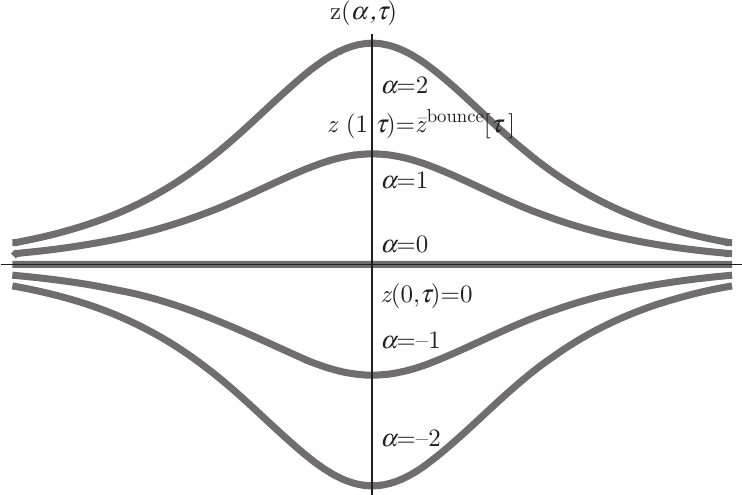
\includegraphics[scale= 0.3]{FIGURAS/trayectorias}
%		\caption{}
%		\label{fig:trayectorias}
%	\end{subfigure}
%	\hfill
%	\begin{subfigure}[t]{0.5\textwidth}
%		\centering
%		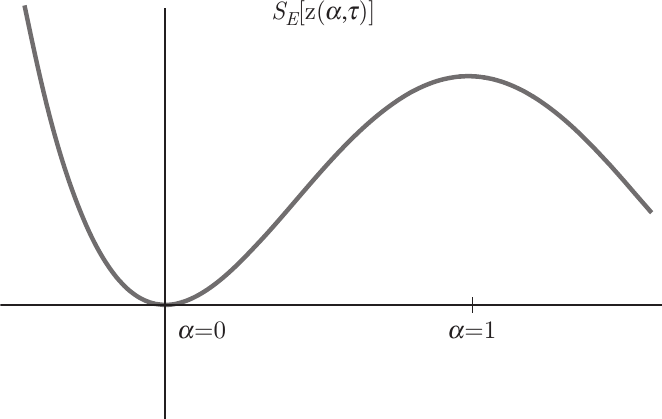
\includegraphics[scale= 0.3]{FIGURAS/accion}
%		\caption{}
%		\label{fig:accion}
%	\end{subfigure}
%	\caption{(a) Algunas de las trayectorias a lo largo del contorno en el espacio de trayectorias parametrizada por $\alpha$. (b) Comportamiento de $S\qty(\alpha)$ a lo largo del mismo contorno. En ambas figuras, $z\qty(\alpha, \tau)$ se corresponde con $x\qty(\alpha, \tau)$ \cite{paranjape2017theory}.}
%\end{figure}
%
%%Por otro lado, sabemos que al ser una trayectoria clásica, %el bounce es un mínimo, por lo que en realidad el bounce es un punto de silla. 
%
%%tal que $S\qty(\alpha)$ tiene el mismo comportamiento que la acción euclideana a lo largo de esta
%
%Para solucionar este problema es necesario deformar el contorno de integración al plano complejo. A partir de $\alpha = 1$ se sigue el contorno de máximo descenso (\emph{steepest descent}) de $-S\qty(\alpha)$
%
%Generalizando el análisis anterior a la integral de camino euclideana

\end{itemize}

\subsection{Multibounce}

\begin{itemize}
	
	\item Debido a la invariancia ante translaciones temporales en el caso $T \rightarrow \infty$ existe una familia de configuraciones dependientes de un parámetro que corresponden a bounces ocurriendo en todo tiempo en $\tau_0 \in \qty[-T/2, T/2]$. Su acción es exponencialmente cerca a $S_B$. Su degeneración es $T$. También existen $n$ bounces separados por un tiempo con acción  exponencialmente cerca a $nS_B$ . Su degeneración es $T^n/n!$ al ser análogos a partículas identicas \cite{paranjape2017theory}.
	
\end{itemize}

\section{Decaimiento del falso vacío en la Teoría Cuántica de Campos}

\begin{itemize}
\item La ocurrencia de los modos cero esta asociado con el hecho de que el centro del bounce puede localizarse en cualquier punto del espaciotiempo euclideano \cite{rubakov2009classical}. 
\end{itemize}

\section{Conclusiones}

\begin{itemize}

\item  Si bien hemos podido calcular la tasa de decaimiento del falso vacío para el campo escalar haciendo uso de la integral de camino euclideana y la aproximación de punto estacionario, tal como lo propusieron Callan y Coleman, aún quedan ciertas ambigüedades conceptuales  ser resueltas. Por ejemplo, ¿como entender el tunelamiento, un proceso dinámico, a partir de una ecuación estática? ¿Cómo puede tener la energía del estado metaestable una parte imaginaria sin estar en contradicción con la hermiticidad? ¿Es posible entender el tunelamiento usando la integral de camino en tiempo real? \cite{Ai:2019dqr}

\printbibliography
\addcontentsline{toc}{chapter}{Bibliografía}

\end{itemize}

\end{document}